\chapter{Results}


% 1)document search 2)workflow search 3)permission 4)detail of workflow and document

% source code structure
\section{Source Code Structure}
\begin{figure}[h!]
	\Large
	\centering
	\caption{Source code structure of this project.}
	\label{fig:source-code-structure}
	\begin{minipage}{6cm}\dirtree{%
			.1 monkeyOffice.
			.2 config.
			.2 lib.
			.2 middleware.
			.2 model.
			.3 document.
			.2 public.
			.3 font-awesome.
			.3 fonts.
			.3 images.
			.3 javascripts.
			.3 stylesheets.
			.4 dist.
			.5 css.
			.5 js.
			.4 login.
			.2 routes.
			.3 api.
			.3 download.
		}
	\end{minipage}
		\begin{minipage}{6cm}\dirtree{%
				.1 monkeyOffice.
				.2 test.
				.3 integration.
				.4 routing.
				.5 api.
				.3 unittest.
				.4 model.
				.5 document.
				.2 uploads.
				.2 utility.
				.2 views.
				.3 dms.
				.3 errors.
				.3 layouts.
			}
		\end{minipage}
\end{figure}

\newpage 

From \ref{fig:screenshot_login}, at first time user have click the sign up link to create a new account for accessing into the main system which is another page \ref{fig:screenshot_signup}


\begin{figure}[h!]

	\centering
	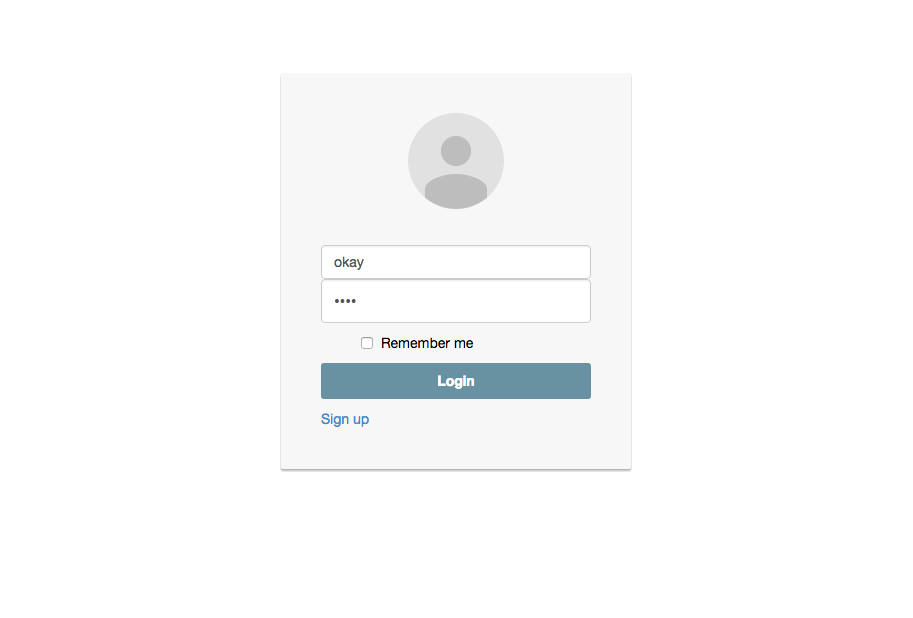
\includegraphics[scale=0.4]{res/Screen_Shot1}
	\caption{Log in page on website}
	\label{fig:screenshot_login}
\end{figure}


\begin{figure}[h!]

	\centering
	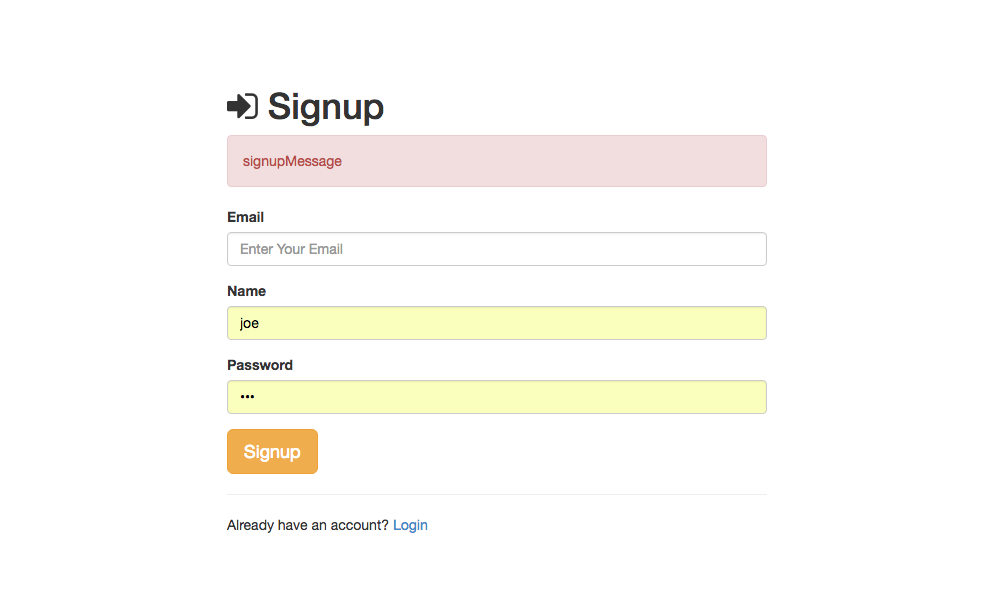
\includegraphics[scale=0.4]{res/Screen_Shot3}
	\caption{Sign up page on website}
	\label{fig:screenshot_signup}
\end{figure}



\begin{figure}[h!]

	\centering
	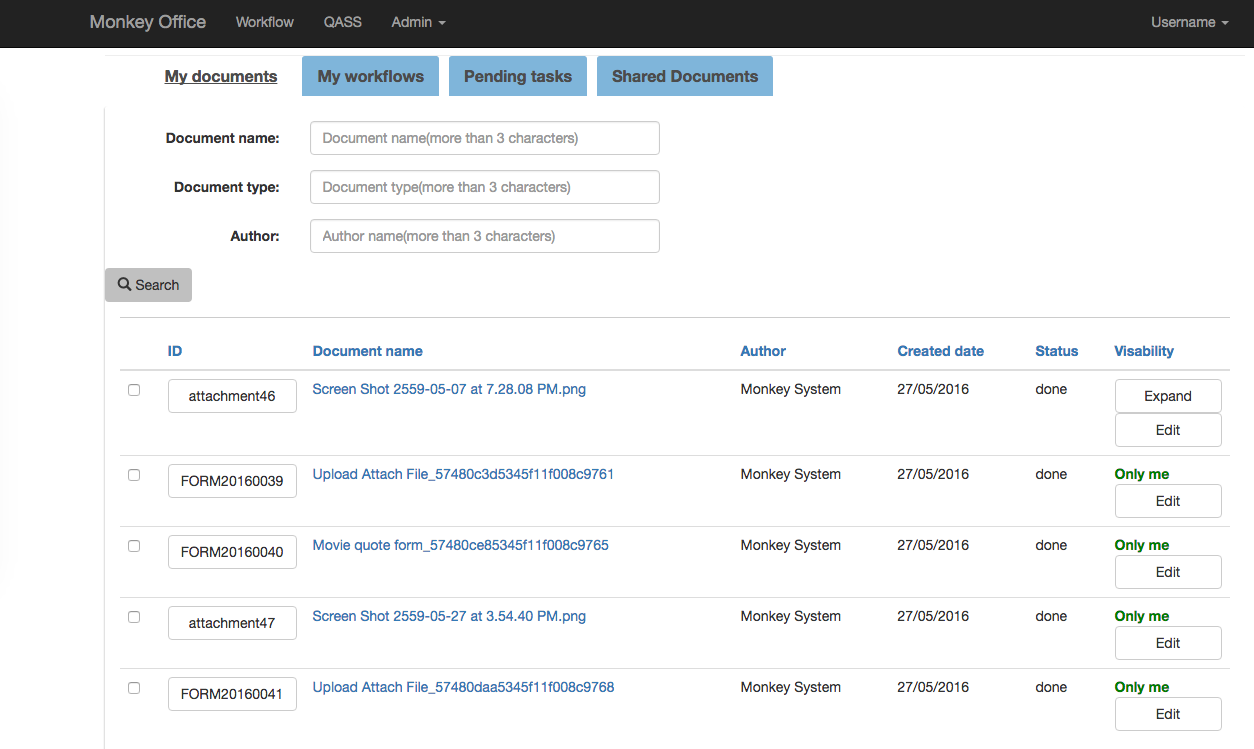
\includegraphics[scale=0.3]{res/home_page}
	\caption{Home page on website}
	\label{fig:screenshot_home}
\end{figure}

\begin{figure}[h!]

	\centering
	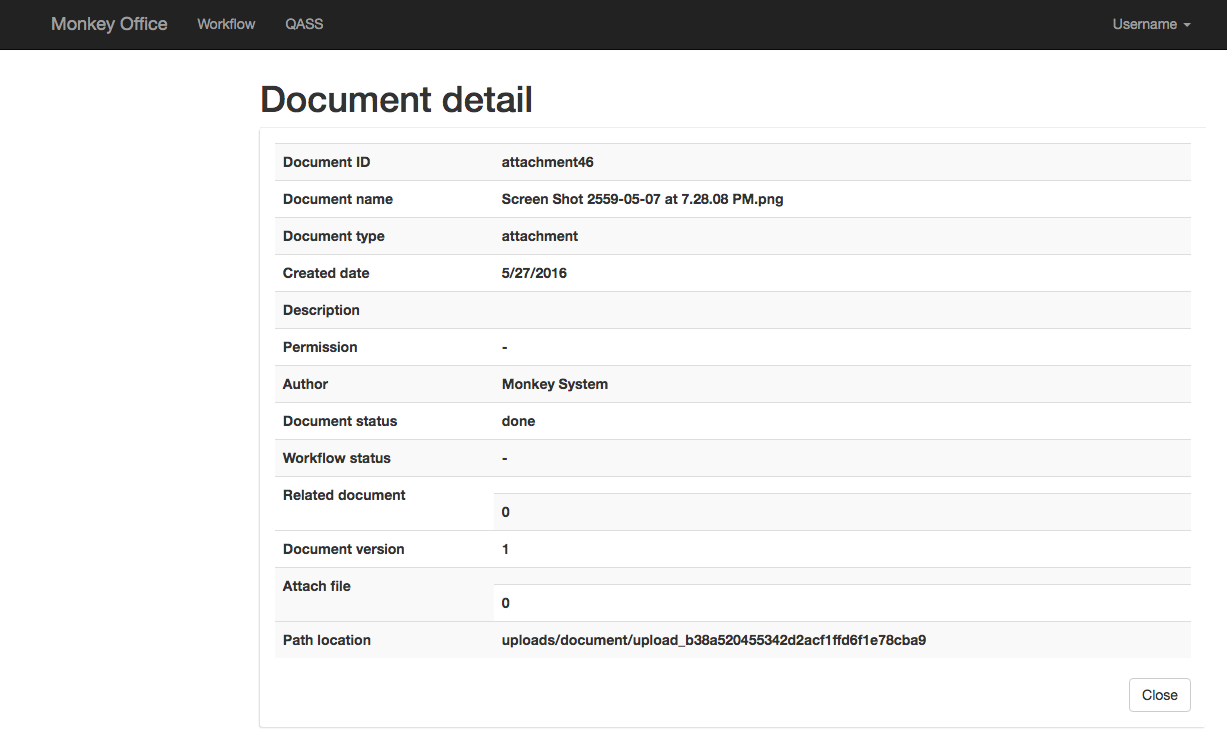
\includegraphics[scale=0.3]{res/doc_detail_page}
	\caption{Document detail page on website}
	\label{fig:screenshot_docdetail}
\end{figure}

\begin{figure}[h!]

	\centering
	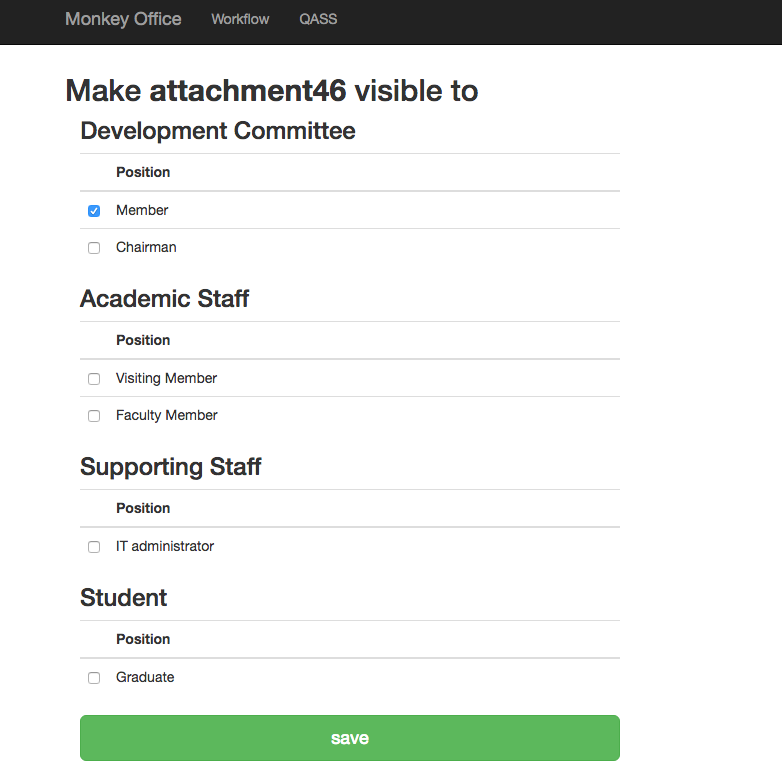
\includegraphics[scale=0.3]{res/permission_page}
	\caption{Permission page on website}
	\label{fig:screenshot_permission}
\end{figure}


After that when the user logged in 	user can see the tabs of documents, workflows, pending tasks and shared document. On my document tab, user can click view detail of document to get more information of document file and click to download the file on link name that user selected, user can searching the documents by name of document, author name and type of document. Moreover, user can edit the permission of each user's document \ref{fig:screenshot_home}, \ref{fig:screenshot_docdetail} and \ref{fig:screenshot_permission}

\begin{figure}[h!]

	\centering
	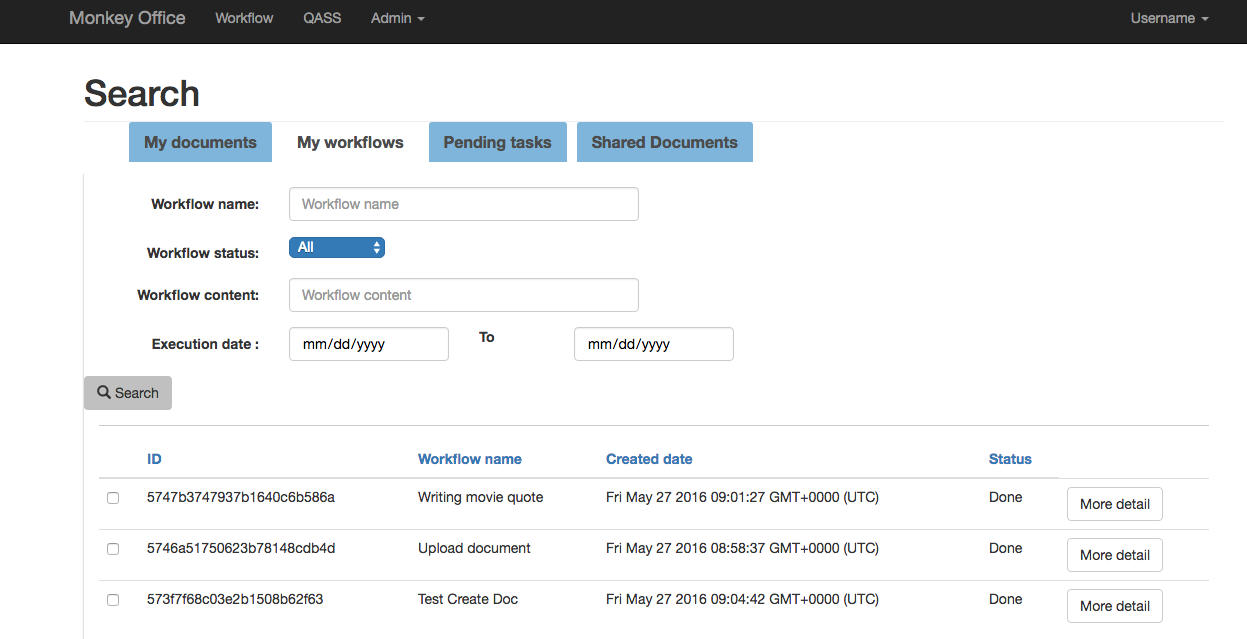
\includegraphics[scale=0.3]{res/tab_wf_page}
	\caption{Tab workflow in home page}
	\label{fig:screenshot_tabwf}
\end{figure}

\begin{figure}[h!]

	\centering
	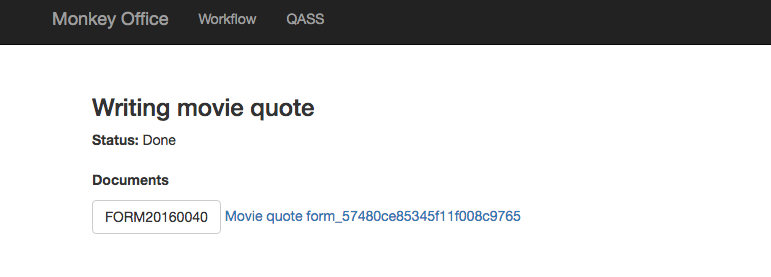
\includegraphics[scale=0.3]{res/wf_detail_page}
	\caption{Workflow detail page on website}
	\label{fig:screenshot_wfdetail}
\end{figure}

\begin{figure}[h!]

	\centering
	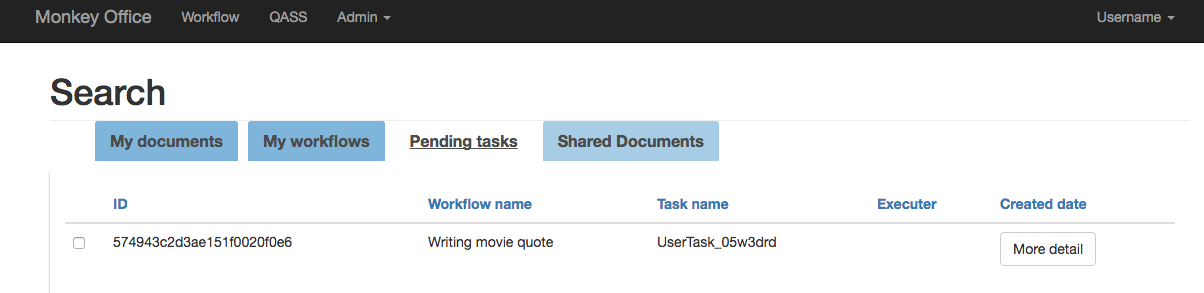
\includegraphics[scale=0.3]{res/pending_page}
	\caption{Tab pending task in home page}
	\label{fig:screenshot_pending}
\end{figure}

 On workflow tab user can search workflow by name, status, any content in workflow and execution date, user also can click to look more detail to go the workflow page that user selected file and pending task tab user can do only look more detail to do the task following workflow rule. \ref{fig:screenshot_tebwf}, \ref{fig:screenshot_wfdetail} and \ref{fig:screenshot_pending}

 \begin{figure}[h!]

	\centering
	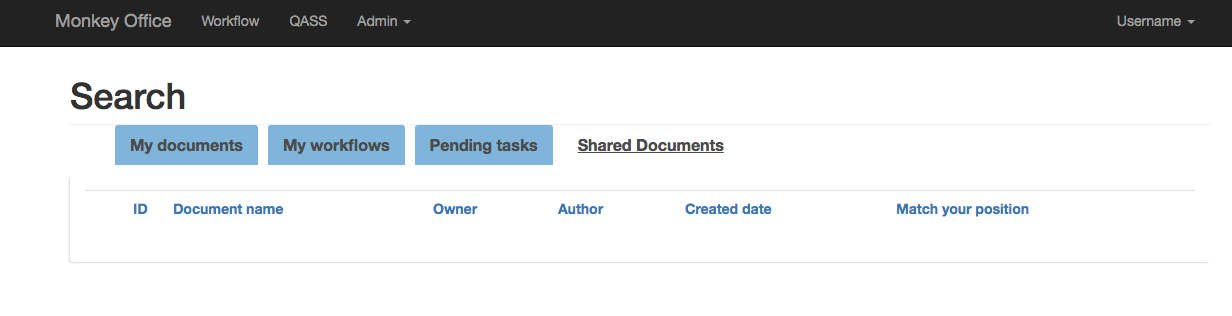
\includegraphics[scale=0.3]{res/tab_shared_page}
	\caption{Tab shared document in home page}
	\label{fig:screenshot_shared}
\end{figure}

At last, shared document tab is different from other because user can do only click to download file in any type of attach files or document files. \ref{fig:screenshot_shared}

% tour the interface

% demonstration

% testing

